\chapter{Structural graph theory}

\section{Minors and subgraphs}

\begin{defn}
	$H \leq_{t} G$ means that subdivision of $H$ is a subgraph of $G$, also known as \textbf{topological minor}.
\end{defn}

\begin{defn}
	$H \leq_{m} G$ means that $H$ is a \textbf{minor} of $G$.
\end{defn}

\begin{defn}
	$H \subseteq G$ means that $H$ is a \textbf{subgraph} of $G$.
\end{defn}

\begin{defn}
	$H \sqsubseteq G$ means that $H$ is a \textbf{induced subgraph} of $G$.
\end{defn}

\begin{thm}[Kuratowski]
	$$
	K_{5}, K_{3,3} \nleq_{t} G \Leftrightarrow G \text{ planar}
	$$
	
	$$
	K_{5}, K_{3,3} \nleq_{m} G \Leftrightarrow G \text{ planar}
	$$
\end{thm}

\begin{defn}
	$\chi(G)$ means that $G$ has a coloring of size $\chi(G)$.
\end{defn}

\begin{observ}
	$C_{3}, C_{5}, C_{7}, \dots \nsubseteq G \Leftrightarrow \chi(G) \leq 2$ which holds also for $\sqsubseteq$.
\end{observ}

\begin{observ}
	$C_{3} \nleq_{m} G \Leftrightarrow G \text{ is a forest}$ also holds for $\leq_{t}$.
\end{observ}

\begin{defn}
	$Forb_{\leq} (\mathcal{F}) = \{G | (\forall F \in \mathcal{F}) F \nleq G\}$
\end{defn}

We will try to show $\mathcal{G} = Forb_{\leq_{m}} (\mathcal{F})$. If $G \in \mathcal{G}$ then all minors of $G$ belong to $\mathcal{G}$.

\begin{observ}
	If $\mathcal{G} = Forb_{\leq}(\mathcal{F})$ then $\mathcal{G}$ is $\leq$-closed. Which means that $\forall G,G'$ if $G \in \mathcal{G}$ and $G' \leq G$ then $G' \in \mathcal{G}$.
\end{observ}

\begin{lemma}
	Let $\leq$ be a partial ordering of graphs. If a class $\mathcal{G}$ of graphs is $\leq$-closed, then there exist $\mathcal{F}$ s.t. $\mathcal{G} = Forb_{\leq}(\mathcal{F})$.
\end{lemma}

\begin{proof}
	$\mathcal{F} = \{F : F \nleq G\}$.
\end{proof}

\begin{defn}
	$F$ is \textbf{minimal $\leq$-obstruction} for $\mathcal{G}$ if $F \notin \mathcal{G}$ but for every $F' \lneq F$ and $F' \in \mathcal{G}$.
\end{defn}

\begin{lemma}
	Let $\leq$ be an ordering of graphs \textbf{without infinite decreasing chains}. If $\mathcal{G}$ is $\leq$-closed, then $\mathcal{G} = Forb_{\leq}(\{F : F \text{ is a minimal } \leq\text{-obstruction for } \mathcal{G}\})$.
\end{lemma}

\begin{proof}
	$G \notin \mathcal{G}$ is min $\leq$-obstruction or $\exists G' \lneq G : G \notin \mathcal{G} \Rightarrow G'$ is obstruction or we continue and because we don't have \textbf{infinite decreasing chains} we will eventually end.
\end{proof}

If $\mathcal{G}$ is $\leq_{m}$-closed, then there exists a \textbf{finite} $\mathcal{F}$ such that $\mathcal{G} = Forb_{\leq_{m}}(\mathcal{F})$.

\begin{thm}[Robertson-Seymor]
	For every $F$ there exists an algorithm that for input graph $G$ decides whether $F \leq_{m} G$ in time $O_{F}(|G|^{3})$.
\end{thm}

\begin{defn}
	For graph $G = (V,E)$ we define $|G| := |V|$ and $||G|| := |E|$. Also for some $U \subseteq V$ $G[U]$ is a induced subgraph of $G$ that has only vertices from $U$. Then $N_{G}(v)$ stands for the neighborhood of vertex $v$ in graph $G$.
\end{defn}

\begin{defn}
	$G'$ is a \textbf{cover} of $G$ if $(\exists f : V(G') \to V(G)) \forall v \in V(G')$ for $N_{G'}(v)$ is a bijection with $N_{G}(f(v))$.
\end{defn}

\begin{example}
	We may see an example \ref{covers}:
	\begin{figure}[!h]\centering
		\begin{subfigure}{0.4\textwidth}\centering
			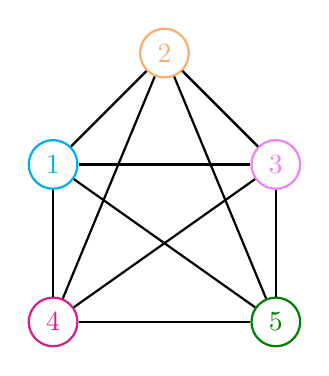
\begin{tikzpicture}[node distance={20mm}, thick, main/.style = {draw, circle}]
				\node[main, color = cyan] (1) {1};
				\node[main, color = Apricot, above right of = 1] (2) {2};
				\node[main, color = Violet, below right of=2] (3) {3};
				\node[main, color = VioletRed, below of=1] (4) {4};
				\node[main, color = Green, below of = 3] (5) {5};
				\path (1) edge (2)
					(1) edge (3)
					(1) edge (5)
					(2) edge (3)
					(2) edge (3)
					(2) edge (4)
					(2) edge (5)
					(3) edge (4)
					(4) edge (5)
					(1) edge (4)
					(3) edge (5);
			\end{tikzpicture}
			\caption{Original graph $G$.}
		\end{subfigure}
		\begin{subfigure}{0.55\textwidth}\centering
			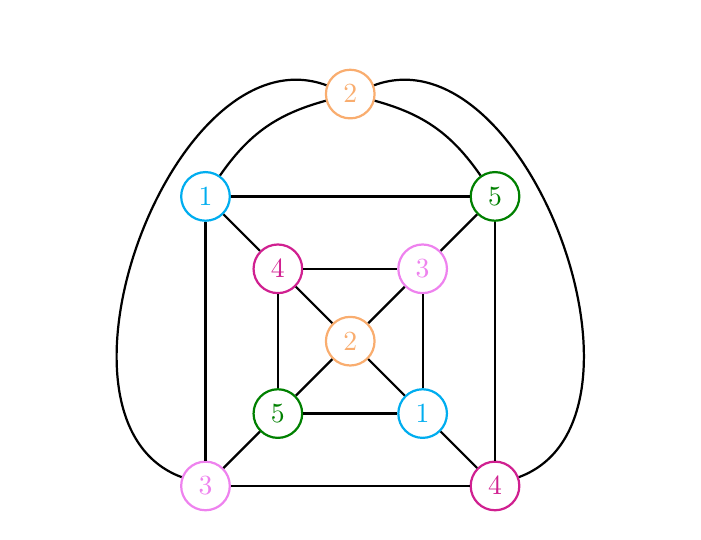
\begin{tikzpicture}[node distance={13mm}, thick, main/.style = {draw, circle}]
				\node[main, color = cyan] (6) {1};
				\node[main, color = VioletRed, below right of = 6] (7) {4};
				\node[main, color = Apricot, below right of = 7] (8) {2};
				\node[main, color = cyan, below right of = 8] (9) {1};
				\node[main, color = VioletRed, below right of=9] (10) {4};
				\node[main, color = Green, below left of=8] (11) {5};
				\node[main, color = Violet, below left of=11] (12) {3};
				\node[main, color = Violet, above right of=8] (13) {3};
				\node[main, color = Green, above right of=13] (14) {5};
				\node[main, color = Apricot, above right of=6, above left of=14, above of=8] (15) {2};
				\path (6) edge (7)
					(7) edge (8)
					(8) edge (9)
					(8) edge (11)
					(8) edge (13)
					(9) edge (10)
					(11) edge (12)
					(13) edge (14)
					(7) edge (13)
					(13) edge (9)
					(9) edge (11)
					(11) edge (7)
					(6) edge (14)
					(14) edge (10)
					(10) edge (12)
					(12) edge (6);
				\path (6) edge [bend left = 20] (15)
					(14) edge [bend right = 20] (15)
					(10) edge [bend right = 90] (15)
					(12) edge [bend left = 90] (15);
			\end{tikzpicture}
			\caption{Cover graph $G'$.}
		\end{subfigure}
		\caption{Example of $G$ and $G'$ as covers.}
		\label{covers}
	\end{figure}
\end{example}

$$
\begin{array}{c}
	\{G | \exists \text{ planar } G' \text{ cover of } G \} \\
	\Updownarrow \\
	F_{1}, \dots, F_{n} \nleq_{m} G
\end{array}
$$

Contrary we take $\mathcal{G} = \{G : (\forall uv \in V(G) \ u \neq v, \deg(u) \geq 5, \deg(v) \geq 5) (\exists X \subseteq E(G) : |X| \leq 1) \ u \text{ and } v \text{ are in different component of } G - X\}$ which is $\leq_{t}$-closed. But take these graphs:

\begin{figure}[!h]\centering
	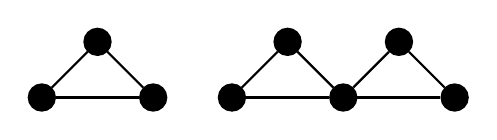
\begin{tikzpicture}[node distance={10mm}, thick, main/.style = {draw, circle, fill}]
		\node[main] (1) {};
		\node[main] (2) [above right of=1] {};
		\node[main] (3) [below right of=2] {};
		\node[main] (4) [right of=3] {};
		\node[main] (5) [above right of=4] {};
		\node[main] (6) [below right of=5] {};
		\node[main] (7) [above right of=6] {};
		\node[main] (8) [below right of=7] {};
		\path
			(1) edge [above] (2)
			(2) edge [above] (3)
			(1) edge [below] (3);
		\path
			(4) edge (5)
			(5) edge (6)
			(6) edge (7)
			(7) edge (8)
			(4) edge (6)
			(6) edge (8);
	\end{tikzpicture}
	\label{endless}
	\caption{Obstructions.}
\end{figure}

Where each one of them is an obstruction. And we could create much more of them.

Now we take a look at some nice properties of graphs if we forbid some graphs as a minors.

$$
\begin{array}{r c l}
	K_{1} \nleq_{m} G & \Leftrightarrow & V(G) = \emptyset \\
	K_{2} \nleq_{m} G & \Leftrightarrow & E(G) = \emptyset \\
	K_{3} \nleq_{m} G & \Leftrightarrow & G \text{ is a forest } \\
	                  &                 & G \text{ is obtained from } K_{1}, K_{2} \text{ by clique sums} \\
	K_{4} \nleq_{m} G & \Leftrightarrow & G \text{ is obtained from } K_{1}, K_{2}, K_{3} \text{ by clique sums} \\
\end{array}
$$

\section{Clique sums}

\begin{defn}
	Graph $G$ can be obtained from $G_{1}$ and $G_{2}$ by \textbf{clique-sum} if the inter-\newline section that these graphs have in $G$ form a clique. In other way it is that we bind together two graphs by identifying their vertices and edges in the same size clique. Sometimes we may denote it as $G_{1} \bigoplus G_{2} = G$. Or even $G_{1} \bigoplus_k G_{2} = G$ to explicitly state the size of the clique is $k$.
\end{defn}

\begin{observ}
	If $G$ is obtained from $G_{1}$ and $G_{2}$ by a clique-sum then:
	
	$$
	K_{m} \leq_{m} G \Leftrightarrow K_{m} \leq_{m} G_{1} \lor K_{m} \leq_{m} G_{2}
	$$
\end{observ}

\begin{lemma}
	If $K_{k} \leq_{m} G$ and $G$ is the clique-sum of $G_{1}$ and $G_{2}$ then $K_{k} \leq_{m} G_{1} \lor K_{k} \leq_{m} G_{2}$.
\end{lemma}

\begin{lemma}
	If $G$ is not $3$-connected then there exist $G_{1}, G_{2} \lneq_{m} G$ s.t. $G$ is a clique-sum of $G_{1}$ and $G_{2}$.
\end{lemma}

\begin{proof}
	If $G$ is not connected then it is done since it is a clique sum on $K_{0}$. If $G$ is connected, but not $2$-connected then it is a clique-sum on $K_{1}$ since there exist a articulation. If $G$ is $2$-connected then there must be two vertices which splits the graph. And these two vertices form a $K_{2}$ as a minor. That is because we split $G$ to two parts where we leave the major one side and add a edge to these two vertices, which we can do because they need to have a path between them so we contract all the edges alongside the path.
\end{proof}

\begin{defn}
	$\delta(G)$ is a minimum degree of a graph $G$.
\end{defn}

\begin{thm}
	If $G$ is $K_{4}$-minor-free then $G$ is obtained from $K_{\leq 3}$'s by clique-sums.
\end{thm}

\begin{proof}
	By induction on $|V(G)|$.
	
	\begin{enumerate}[(a)]
		\item If $G$ is not 3-connected. $G$ is a clique-sum of $G_{1},G_{2} \lneq_{m} G$. Since $K_{4} \nleq_{m} G_{1}$ and $K_{4} \nleq_{m} G_{2}$ we use induction hypothesis and we are done.
		\item If $G$ is 3-connected. If $|V(G)| \leq 3$, then $G = K_{\leq 3}$, wlog $|V(G)| \geq 4$. $\delta(G) > 1 \Rightarrow G$ contains a cycle. Let $C$ be the shortest cycle in $G$. $C$ is induced in $G$ 3-connected $\Rightarrow G \neq C$ so $\exists v \in V(G) \setminus V(C)$. By Merger's theorem there exists three paths from $v$ to $C$ intersecting only in $v$. That gives us $K_{4}$ as a minor of the graph. Which is contradiction.
	\end{enumerate}
\end{proof}

$$
\begin{array}{r c l}
	K_{5} \nleq_{m} G & \Leftrightarrow & G \text{ is obtained from planar graphs and } W_{8}  \text{ by clique sums} \\
\end{array}
$$

\begin{figure}[!h]\centering
	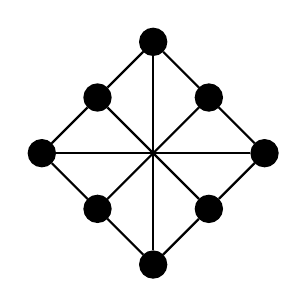
\begin{tikzpicture}[node distance={10mm}, thick, main/.style = {draw, circle, fill}]
		\node[main] (1) {};
		\node[main] (2) [above right of=1] {};
		\node[main] (3) [below right of=2] {};
		\node[main] (4) [below left of=1] {};
		\node[main] (5) [below right of=3] {};
		\node[main] (6) [below left of=5] {};
		\node[main] (7) [below right of=4] {};
		\node[main] (8) [below right of=7] {};
		\draw (1) -- (2);
		\draw (4) -- (1);
		\draw (4) -- (7);
		\draw (7) -- (8);
		\draw (8) -- (6);
		\draw (6) -- (5);
		\draw (3) -- (5);
		\draw (2) -- (3);
		\draw (2) -- (8);
		\draw (1) -- (6);
		\draw (4) -- (5);
		\draw (7) -- (3);
	\end{tikzpicture}
	\caption{$W_{8}$ graph.}
	\label{w8}
\end{figure}

\begin{observ}
	If $G$ is a clique-sum of $G_{1}$ and $G_{2}$ then
	
	$$
	\chi(G) \leq \max (\chi(G_{1}), \chi(G_{2}))
	$$
\end{observ}

\begin{proof}
	We just need to match the coloring of the cliques. Other than that we don't have any problem.
\end{proof}

\section{Hadwiger's conjecture}

$K_{t}$-minor-free graphs are $(t-1)$ colorable.

$$
\begin{array}{c c c}
	K_{1} \nleq_{m} G & \chi \leq 1 & \delta \leq 0 \\
	K_{2} \nleq_{m} G & \chi \leq 2 & \delta \leq 1 \\
	K_{3} \nleq_{m} G & \chi \leq 3 & \delta \leq 2 \\
	K_{4} \nleq_{m} G & \chi \leq 4 & \delta \leq 5 \\
	K_{5} \nleq_{m} G & \chi \leq 5 & \\
\end{array}
$$

\begin{thm}
	$\exists f$ every $K_{t}$-minor-free graph $G$ has $\delta(G) \leq f(t)$.
\end{thm}

The function is somewhere near $f(t) = (1,6\dots + O(1)) t \sqrt{\log t}$. But we won't show this result. Instead we will show $f(t) = O(t^{2})$.

\section{Chordal decomposition}

Before we continue it is better to remind ourselves \textbf{chordal graph} and \textbf{elimination ordering} (known as PES).

\begin{defn}[Chordal decomposition of $G$]
	$V(G) = \mathcal{P}_{1} \dot{\cup} \mathcal{P}_{2} \dot{\cup} \dots \dot{\cup} \mathcal{P}_{n}$ and
	
	\begin{enumerate}
		\item $(\forall i) G[\mathcal{P}_{i}]$ is connected.
		\item "$\mathcal{P}_{i}$'s form elimination ordering" Precisely: $(\forall i \in [n])(\forall j_{1},j_{2} < i)$ if $G$ has an edge between $\mathcal{P}_{i}$ and $\mathcal{P}_{j_{1}}$ and also between $\mathcal{P}_{i}$ and $\mathcal{P}_{j_{2}}$ then it also has an edge between $\mathcal{P}_{j_{1}}$ and $\mathcal{P}_{j_{2}}$.
	\end{enumerate}
\end{defn}

\begin{defn}
	Chordal partition is \textbf{geodesic} if $(\forall i) (\exists v_{i} \in \mathcal{P}_{i})$ s.t. if $j_{1}, \dots, j_{t} < i$ are the indices s.t. $G$ has an edge between $\mathcal{P}_{i}$ and $\mathcal{P}_{j_{1}}, \mathcal{P}_{j_{2}}, \dots, \mathcal{P}_{j_{t}}$ then $u_{1}, \dots, u_{t} \in \mathcal{P}_{i}$ s.t. $u_{i}$ has a neighbor in $\mathcal{P}_{j_{1}}, \mathcal{P}_{j_{2}}, \dots, \mathcal{P}_{j_{t}}$ and $G - \bigcup_{j < i} \mathcal{P}_{j}$ contains shortest paths from $v_{i}$ to $u_{1}, \dots, u_{t}$ which cover all vertices in $\mathcal{P}_{i}$.
\end{defn}

% TODO perhaps add an image

\begin{thm}
	Every graph has a geodesic chordal partition.
	\label{geodesic-thm}
\end{thm}

Before we show us the proof we will take a look at a simple application. If $G$ is $K_{k}$-minor-free last part has neighbours in $t \leq k-2$ parts (otherwise it will have $K_{k}$ as a minor). Then we may take a look at a $\deg(v) \leq (k-2) + (k-2)(k-2)3 \leq 3k^{2}$. Thus getting the upper bound $\delta(G) \leq 3k^{2}$.

\begin{defn}
	Part is called \textbf{terminal} if there is no edge from any vertex in that part going to some vertex in one of the parts on the right.
\end{defn}

\begin{proof}[Proof of theorem \ref{geodesic-thm}]
	Let $\mathcal{P}$ be a chordal decomposition of $G$ into parts satisfying both properties of definition of chordal decomposition (i) and (ii) and geodesity (iii) for all non-terminal parts.
	
	This can be easily done by creating parts based on the components of connectivity. For them all properties hold, since they are all connected and "chordal" property is also satisfied since there are no edges. Also all of them are terminal (iii) doesn't have to be satisfied.
	
	Now we proof that by choosing $\mathcal{P}$ with largest number of parts. Lets say that there is a part that does not satisfy (iii). This means that it is terminal part. Lets take vertex from the part and find the shortest paths to the vertices that are connected to some of the parts to the left. Now we put vertices to separate components and these components will make a new parts. We will also remove all these vertices from the origin part. Note that all properties are satisfied. (i) is trivial. (ii) If there are any vertices from the new parts to other parts then they are to the ones which are already connected to the origin part, which satisfied (ii) before so it is fine. Also (iii) is satisfied.
	
	The thing is that we created $\mathcal{P}$ with larger number of parts which is contradiction.
\end{proof}

\begin{observ}
	$H \leq_{t} G \Rightarrow H \leq_{m} G$
\end{observ}

\begin{observ}
	$\Delta (H) \leq 3 : H \leq_{m} G \Rightarrow H \leq_{t} G$
\end{observ}

Lets remind ourselves a table and add some new properties.

$$
\begin{array}{ r c l}
	K_{1} \nleq_{t} G \Leftrightarrow K_{1} \nleq_{m} G & \Leftrightarrow & V(G) = \emptyset \\
	K_{2} \nleq_{t} G \Leftrightarrow K_{2} \nleq_{m} G & \Leftrightarrow & E(G) = \emptyset \\
	K_{3} \nleq_{t} G \Leftrightarrow K_{3} \nleq_{m} G & \Leftrightarrow & G \text{ is a forest } \\
	&                 & G \text{ is obtained from } K_{1}, K_{2} \text{ by clique sums} \\
	K_{4} \nleq_{t} G \Leftrightarrow K_{4} \nleq_{m} G & \Leftrightarrow & G \text{ is obtained from } K_{1}, K_{2}, K_{3} \text{ by clique sums} \\
	K_{5} \nleq_{t} G \nLeftrightarrow K_{5} \nleq_{m} G & \Leftrightarrow & G \text{ is obtained from planar graphs and } W_{8}  \text{ by clique sums} \\
\end{array}
$$

Well technically $K_{5} \nleq_{t} G \Rightarrow K_{5} \nleq_{m} G$ but the other way around is what doesn't work $K_{5} \nleq_{m} G \nRightarrow K_{5} \nleq_{t} G$. For that we can see an example \ref{minor-not-top}. We may see that $\mathcal{G} = \{G : G \text{ has } \leq 4 \text{ vertices of degree } \geq 4\}$ these graphs are so that $K_{5} \nleq_{t} G$.

\begin{figure}[!ht]\centering
	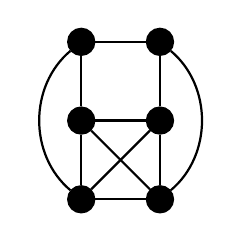
\begin{tikzpicture}[node distance={10mm}, thick, main/.style = {draw, circle, fill}]
		\node[main] (1) {};
		\node[main] (2) [right of=1] {};
		\node[main] (3) [below of=1] {};
		\node[main] (4) [below of=2] {};
		\node[main] (5) [below of=3] {};
		\node[main] (6) [below of=4] {};
		\draw (1) -- (2);
		\draw (1) -- (3);
		\draw (4) -- (2);
		\draw (3) -- (4);
		\draw (5) -- (4);
		\draw (6) -- (4);
		\draw (6) -- (5);
		\draw (3) -- (5);
		\draw (3) -- (6);
		\path
			(1) edge [bend right = 50] (5)
			(2) edge [bend left = 50] (6);
	\end{tikzpicture}
	\caption{A counter example.}
	\label{minor-not-top}
\end{figure}

\section{Hájos conjecture}

If we remember Headwiger's conjecture then Hájos conjecture is the same only with topological minors. Thus it is that $K_{t} \nleq_{t} G \Rightarrow \chi(G) \leq t-1$. This is actually true for $t < 4$ but it is false for $t \geq 7$ and $5,6$ are open questions.

\begin{thm}
	$\exists f_{m}(k) = O(k \sqrt{\log k})$ Every $K_{k}$-minor-free graph $G$ satisfies $\delta(k) \leq f_{m}(k)$.
\end{thm}

We won't prove this, but we will prove something similiar, that is for topological minors.

\begin{thm}
	$\exists f_{t}(k) = O(k^{2})$ Every $G$ s.t. $K_{k} \nleq_{t} G$ satisfies $\delta(G) \leq f_{t}(k)$.
\end{thm}

The corollary to this is that $\chi(G) \leq f_{t}(k) +1$. We will proof this theorem, but to do that we need to do some steps beforehand.

Firstly imagine that the enemy gives you a graph and you need to prove that. But the enemy is kind enough to give you a graph $H$ with connectivity $>> k^2$. We could apply Merger's theorem. Though this will only give certain number of vertex disjoint paths from one vertex to another. We would more likely have this many paths between more pairs of sources and targets.

\section{$k$-linked, model, separation}

\begin{defn}
	Graph $G$ is \textbf{$k$-linked} if $|V(G)| \geq 2k$ and $\forall s_{1}, s_{2}, \dots, s_{k}, t_{1}, t_{2}, t_{k}$ distinct vertices of $G$. $G$ contains pairwise vertex-disjoint paths $P_{1}, P_{2}, \dots, P_{k}$. When $P_{i}$ has ends $s_{i}$ and $t_{i}$.
\end{defn}

We may see that there exist a graph that is 2-connected and yet not 2-linked. You may see this on the picture \ref{2-linked-2}. Also not even 3-connected graph has to be 2-linked. Which is also on the picture \ref{2-linked-3} (though we can change the vertex inside for any planar graph). We could continue and end up with that not even 5-connectivity forces 2-linked.

\begin{figure}[!ht]\centering
	\begin{subfigure}[b]{0.4\textwidth}\centering
		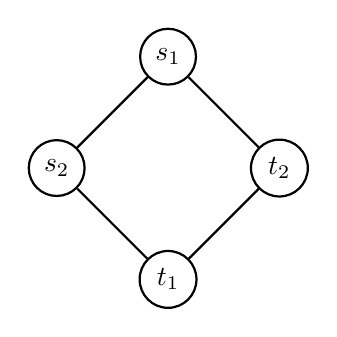
\begin{tikzpicture}[node distance={20mm}, thick, main/.style = {draw, circle}]
			\node[main] (1) {$s_{1}$};
			\node[main] (2) [below left of=1] {$s_{2}$};
			\node[main] (3) [below right of=1] {$t_{2}$};
			\node[main] (4) [below right of=2] {$t_{1}$};
			\draw (1) -- (2);
			\draw (2) -- (4);
			\draw (3) -- (4);
			\draw (3) -- (1);
		\end{tikzpicture}
		\caption{2-connectivity}
		\label{2-linked-2}
	\end{subfigure}
	\begin{subfigure}[b]{0.4\textwidth}\centering
		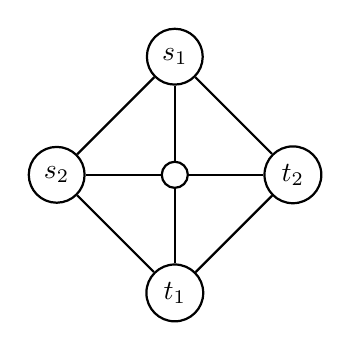
\begin{tikzpicture}[node distance={15mm}, thick, main/.style = {draw, circle}]
			\node[main] (1) {$s_{1}$};
			\node[main, below of=1] (phantom) {};
			\node[main] (2) [left of=phantom] {$s_{2}$};
			\node[main] (3) [right of=phantom] {$t_{2}$};
			\node[main] (4) [below of=phantom] {$t_{1}$};
			\draw (1) -- (2);
			\draw (2) -- (4);
			\draw (3) -- (4);
			\draw (3) -- (1);
			\draw (1) -- (phantom);
			\draw (2) -- (phantom);
			\draw (3) -- (phantom);
			\draw (4) -- (phantom);
		\end{tikzpicture}
		\caption{3-connectivity}
		\label{2-linked-3}
	\end{subfigure}
	\caption{A counter example to 2-linked graphs.}
	\label{2-linked}
\end{figure}

\begin{observ}
	Every $k$-linked graph is $(2k-1)$ connected.
\end{observ}

\begin{proof}
	That is simply because we put all the $s_{i}, t_{i}$ for $i \in [k-1]$ to the vertex cut and then choose $s_{k}$ in the left part and $t_{k}$ in the right part then we can see that it is indeed $(2k-1)$-connected.
\end{proof}

\begin{thm}\label{2-linked-thm}
	If $G$ is $2k$-connected, $K_{4k} \leq_{m} G$ then $G$ is $k$-linked.
\end{thm}

We won't prove this directly. Instead we will later on introduce another theorem that is actually pretty much the same and prove that.

\begin{cor}
	If $G$ is $\max(2k, f_{m}(4k)+1)$-connected then $G$ is $k$-linked.
\end{cor}

\begin{proof}
	We use the theorem to get that $\delta > f_{m}(4k)$ thus $K_{4k} \leq_{m} G$.
\end{proof}

Also we can say $\exists f_{l}(k) = O(k \sqrt{\log k})$. If $G$ is $f_{l}(k)$-connected then $G$ is $k$-linked.

\begin{cor}
	If $G$ is $f_{l}\left( \frac{k (k-1)}{2}\right)$-connected then $K_{k} \leq_{t} G$.
\end{cor}

\begin{proof}
	To see this we choose $k$ vertices and for every one of them $k-1$ neighbors. Then we give $s_{i}$ and $t_{i}$ to every single one of these vertex so that every neighborhood has pair with all others. Then we find such paths between them.
\end{proof}

\begin{lemma}
	If $\bar{d}(G) \geq 4d$ then $G$ contains a $(d+1)$-connected subgraph $H$ of minimum degree $2d+1$.
\end{lemma}

\begin{proof}
	Let $H$ be a minimal subgraph of $G$ s.t. $|V(H)| \geq 2d$ and $|E(H)| > 2d (|V(H)| - d)$. We may see that $|V(H)| > 2d$ that is if it has $2d$ vertices then
	
	$$
	\frac{2d^{2} - d}{2} = \binom{2d}{2} > |E(H)| > 2d^{2}
	$$
	
	which is a contradiction.
	
	Then we also have that $\delta (H) \geq 2d+1$. If we have $\delta(H) \leq 2d$ we may remove the certain vertex. But we need to show that given properties still hold. We will split the graph to two parts $|A|, |B| \geq 2d+2 > 2d$. Then
	
	$$
	\begin{array}{r l}
		|E(G)| & \leq |E(A)| + |E(B)| \\
		(1) & \leq 2d(|V(A)| - d) + 2d(|V(B)| - d) \\
		& = 2d(|V(A)| + |V(B)| - 2d) \\
		& = 2d(|V(H)| - |V(A \cap B)| - 2d) \\
		|E(G)| & > 2d(|V(H)| - d)
	\end{array}
	$$
	
	Where $(1)$ is due to the minimality of $H$. The thing is with the last two lines we get that $|A \cap B| > d$.
\end{proof}

\begin{proof}
	This actually is enough for the theorem to be proven since the enemy doesn't have to be kind anymore.
\end{proof}

\begin{defn}
	A \textbf{model} of $K_{m}$ in $G$ is $M_{1}, M_{2}, \dots, M_{m} \subseteq V(G)$ pairwise distinct and $\forall i : G[M_{i}]$ is connected and $(\forall i \neq j) \exists uv \in E(G): u \in M_{i}, v\in M_{j}$.
\end{defn}

We may take a look at an example of model of $K_{4}$ which is in picture \ref{k4-model}.

\begin{figure}[!ht]\centering
	\begin{tikzpicture}[node distance={10mm}, thick, main/.style = {draw, circle, fill}]
		\node[main] (1) [color=cyan] {};
		\node[main] (2) [above of=1] [color=cyan] {};
		\node[main] (3) [below left of=1] [color=cyan] {};
		\node[main] (4) [below right of=1] [color=cyan] {};
		\node[main] (5) [left of=1] [color=cyan] {};
		\node[main] (6) [right of=1] [color=cyan] {};
		\node[main] (7) [right of=6] [color=cyan] {};
		\node[main] (8) [below right of=6] [below right of=4] [color=orange] {};
		\node[main] (9) [below left of=5] [below left of=3] [color=blue] {};
		\node[main] (10) [left of=9] [color=blue] {};
		\node[main] (11) [below of=10] [color=blue] {};
		\node[main] (12) [below of=9] [color=blue] {};
		\node[main] (13) [below right = 1.8cm of 12] [color=purple] {};
		\node[main] (14) [below left of=13] [color=purple] {};
		\node[main] (15) [below right of=13] [color=purple] {};
		\path[color=blue] (9) edge (10)
			(9) edge (12)
			(10) edge (11)
			(11) edge (12);
		\path[color=cyan] (1) edge (2)
			(1) edge (3)
			(1) edge (4)
			(1) edge (5)
			(1) edge (6)
			(6) edge (7);
		\path[color=purple] (13) edge (14)
			(13) edge (15)
			(14) edge (15);
		\path (8) edge [bend left = 40] (15)
			(8) edge [bend right = 20] (6)
			(8) edge [bend left = 20] (12)
			(13) edge [bend right = 20] (4)
			(14) edge [bend left = 20] (12)
			(10) edge [bend left = 20] (5);
	\end{tikzpicture}
	\caption{Example of $K_{4}$ model.}
	\label{k4-model}
\end{figure}

\begin{observ}
	$K_{m} \leq_{m} G \Leftrightarrow \text{there is a mode of } K_{m} \text{ in } G$.
\end{observ}

\begin{defn}
	\textbf{Separation} in $G$ is $(A,B)$ where $A,B \subseteq V(G), A \cup B = V(G)$, no edge between $A \setminus B$ and $B \setminus A$.
\end{defn}

On picture \ref{separation} we may see an example of $(A,B)$-separation. Where the \textcolor{orange}{orange} points are both in $A$ and $B$ and then the rest is either only in one or second part, which are set by their connectivity.

\begin{figure}[!ht]\centering
	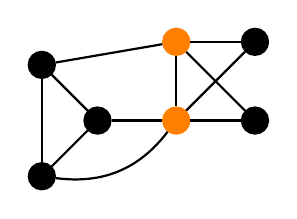
\begin{tikzpicture}[node distance={10mm}, thick, main/.style = {draw, circle, fill}]
		\node[main] (1) [color=orange] {};
		\node[main] (2) [color=orange] [below of=1] {};
		\node[main] (3) [right of=1] {};
		\node[main] (4) [right of=2] {};
		\node[main] (5) [left of=2] {};
		\node[main] (6) [below left of=5] {};
		\node[main] (7) [above left of=5] {};
		\path [thick] (1) edge (2)
		(1) edge (3)
		(1) edge (4)
		(1) edge (7)
		(2) edge (3)
		(2) edge (4)
		(2) edge [bend left = 30] (6)
		(2) edge (5)
		(5) edge (6)
		(5) edge (7)
		(6) edge (7);
	\end{tikzpicture}
	\caption{Example of separation.}
	\label{separation}
\end{figure}

\begin{defn}
	The \textbf{order} of the separation is $|A \cap B|$.
\end{defn}

\begin{defn}
	$S$ is \textbf{well-linked} to a model $M_{1}, M_{2}, \dots, M_{m}$ if every separation $(A,B)$ with $S \subseteq A$ $(\exists i) M_{i} \subseteq B \setminus A$ has order $\geq |S|$.
\end{defn}

\begin{thm}
	$\forall G, S = \{s_{1}, s_{2}, \dots, s_{k}, t_{1}, t_{2}, \dots, t_{k}\} \subseteq V(G)$ and $M_{1}, \dots, M_{4k}$ model of $K_{4k}$ in $G$. If $S$  is well-linked to $M_{1}, M_{2}, \dots, M_{4k}$ then $G$ contains distinct paths from $s_{i}$ to $t_{i}$ for all $i \in [k]$.
\end{thm}

We can see that this is somewhat reformulation of theorem before (\ref{2-linked-thm}). Thus if we prove this we will also prove the previous theorem. But we will introduce another similiar theorem which will imply this theorem.

\begin{defn}
	$G, S \subseteq V(G)$ and $M_{1}, M_{2}, \dots, M_{m} \subseteq V(G)$ pairwise distinct is an \textbf{$S$-relaxed model} of $K_{m}$ in $G$ if
	
	\begin{enumerate}
		\item $(\forall i) G[M_{i}]$ is connected \underline{or} every component of $G[M_{i}]$ intersects $S$.
		\item $(\forall i \neq j) \exists uv \in E(G)$ s.t. $u \in M_{i}, v \in M_{j}$ \underline{or} $M_{i} \cap S \neq \emptyset \neq M_{j} \cap S$.
	\end{enumerate}
\end{defn}

\begin{thm}[\textcolor{Green}{Slightly changed}]
	$\forall G_{i}, S = \{s_{1}, s_{2}, \dots, s_{k}, t_{1}, t_{2}, \dots, t_{k}\} \subseteq V(G)$ and $M_{1}, \dots, M_{4k}$ \textcolor{Green}{$S$-relaxed mdel} of $K_{4m}$ in $G$. If $S$  is well-linked to $M_{1}, M_{2}, \dots, M_{4k}$ then $G$ contains distinct paths from $s_{i}$ to $t_{i}$ for all $i \in [k]$.
\end{thm}

\begin{proof}
	We will prove this theorem by induction on $|V(G)|$. We will separate it to some distinct cases.
	
	\begin{enumerate}[(1)]
		\item Suppose there exisits a separation $(A,B)$ of order $2k$ (which is $= |S|$) s.t. $S \subsetneq A$ and $(\exists i) M_{i} \subseteq B \setminus A$. Then by Menger's theorem there exists $2k$ disjoint paths from $S$ to $A \cap B$ (since $S$ is well-linked to $M_{1}, \dots, M_{4k}$).\textit{ We want: $G[B]$ disjoint paths from $s_{i}'$ to $t_{i}'$ for all $i \in [k]$, where $s_{i}'$ and $t_{i}'$ are the ends from the paths labeled same as the beginings.} We apply induction hypothesis on $G[B]$ $S' = \{s_{i}', t_{i}' | \forall i \in [k]\}$ $M_{1} \cap B, M_{2} \cap B, \dots, M_{4k} \cap B$.
		
		First we need to prove that the properties still holds. Such as that it is still $S'$-relaxed and $S'$ is well-linked. Consider $M_{i} \cap S = \emptyset$ so $\forall j \neq i$ there is at least one vertex in $B$. Then $M_{1} \cap B$ components do not intersect $S'$ so it didn't intersect $S$. Therefore it had to be connected and thus still is. That is the first property and the second is \textit{left out as exercise}. So $S'$ is relaxed model.
		
		We now take a look at if $S'$ wouldn't be well-linked. Then there would be a separation with order $< 2k$. But this separation would be present even before so it cannot be there.
		
		Now WLOG: Every separation $(A,B)$ s.t. $S \subsetneq A, (\exists i) M_{i} \subseteq B \setminus A$ has order $> 2k$.
		
		\item Suppose $\exists v \in V(G) \setminus (S \cup \bigcup_{i}^{4k} M_{i})$ apply I.H. on $G -v$. We need to show that it is well-linked. Suppose we have a separation with order $<2k$. We put $v$ in the intersection of the separation ("cut") and get a separation of $G$ with order $\leq 2k$. That can't happen since we assumed the orrder is $>2k$.
		
		\item Suppose $(\exists i) \exists uv \in E(G[M_{i}])$ s.t. $v \notin S$. Aplly I.H> to $G / uv$ (contract the edge $uv$). We may see that $S$ is relaxed model and well-linked with the similiar arguments as in the point before.
	\end{enumerate}
	
	With this induction we end up with $S \subseteq V(G)$ and $M_{1}, M_{2}, \dots, M_{4k}$. We know $(\forall i) M_{i} \cap S = \emptyset \Rightarrow |M_{i}| =1$ \underline{or} $M_{i} \subseteq S$. Also all single $M_{i}$ forms a clique. We would like to find if there exist a mathcing between $S$ and $V(G) \setminus S$ covering $S$. For that we may recall Hall's theorem and thus we need $\forall X \subseteq S: |N(X)| \geq |X|$ where $N(X)$ are the neighbours of $X$. Lets take a look at one $M_{k} = X$ and its $N(X)$. There are not necessarily edges to $M_{1}, \dots, M_{g}$. Lets put $A = S \cup N(X)$ and $B = \text{ clique on } M_{i}\text{s} \cup (S \setminus X)$. By that we get that $X = A \setminus B$ and $V(G) \setminus (S \cup N(X)) = B \setminus A$. So $(S \setminus X) \cup N(X) = A \cap B$ which can't be smaller than $2k$. So $|S \setminus X| + |N(X)| \geq 2k$ where $S \setminus X| = |S| - |X|$ and $|S| = 2k$ this means that $|N(x)| \geq |X|$.
	
	Therefore we find the matching between $S$ and clique. Thus we take for each $i$ the edge in matching from $s_{i}$ to $s_{i}'$, then path from clique from $s_{i}'$ to $t_{i}'$ and next from matching $t_{i}'$ to $t_{i}$.
\end{proof}